\section{整型数据}


\begin{frame}\ft{整数的存储方式}
数据都是以二进制的形式存储。\vspace{0.1in}

整数以补码的方式存储。\vspace{0.1in}

\begin{enumerate}
\item
正数的补码是其本身\\[0.1in]
\item 
负数的补码:将其绝对值的二进制形式按位取反再加1。
\end{enumerate}
\end{frame}
%
\begin{frame}\ft{整数的存储方式}

\begin{figure}
\centering
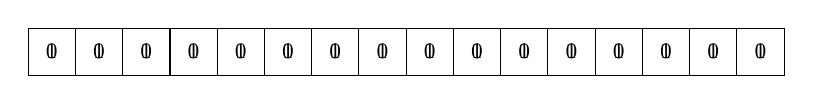
\begin{tikzpicture}
\def\x{0.6}
\foreach \i in {0,1,...,15}{
\draw (-\i*\x,0)rectangle(-\i*\x-\x,\x);
\ifthenelse{\i=1 \OR \i=3}
{
\node at (-\i*\x-0.5*\x,0.5*\x)[]{\footnotesize{1}};
}
{
\node at (-\i*\x-0.5*\x,0.5*\x)[]{\footnotesize{0}};

}
}
\end{tikzpicture}
\caption{正数10的存储方式}
\end{figure}
%
\begin{figure}
\centering
\begin{tikzpicture}
\def\x{0.6}
\foreach \i in {0,1,...,15}{
\draw (-\i*\x,0)rectangle(-\i*\x-\x,\x);
\ifthenelse{\i=1 \OR \i=3}
{
\node at (-\i*\x-0.5*\x,0.5*\x)[]{\footnotesize{1}};
}
{
\node at (-\i*\x-0.5*\x,0.5*\x)[]{\footnotesize{0}};
}
}
\node at (-16*\x,1.3*\x) [right]{\footnotesize{10的原码}};
%%%%
\foreach \i in {0,1,...,15}{
\draw (-\i*\x,-2*\x)rectangle(-\i*\x-\x,-\x);
\ifthenelse{\i=1 \OR \i=3}
{
\node at (-\i*\x-0.5*\x,-1.5*\x)[]{\footnotesize{0}};
}
{
\node at (-\i*\x-0.5*\x,-1.5*\x)[]{\footnotesize{1}};
}
}
\node at (-16*\x,-0.7*\x) [right]{\footnotesize{取反}};
%%%%
\foreach \i in {0,1,...,15}{
\draw (-\i*\x,-4*\x)rectangle(-\i*\x-\x,-3*\x);
\ifthenelse{\i=0 \OR \i=3}
{
\node at (-\i*\x-0.5*\x,-3.5*\x)[]{\footnotesize{0}};
}
{
\node at (-\i*\x-0.5*\x,-3.5*\x)[]{\footnotesize{1}};
}
}
\node at (-16*\x,-2.7*\x) [right]{\footnotesize{加1,得-10的补码}};

\end{tikzpicture}
\caption{负数-10的存储方式}
\end{figure}
\end{frame}
%
\begin{frame}[fragile]\ft{int型}
int型表示有符号整数,其取值范围依赖于系统,可通过以下代码查看。
\end{frame}
%
\begin{frame}[fragile]\ft{int型}
\lstinputlisting[language=C,numbers=left,frame=single]{Code/int_max_min.c}
\end{frame}

\begin{frame}[fragile]\ft{int型}
\begin{lstlisting}[backgroundcolor=\color{red!10}]
$ gcc int_max_min.c
$ ./a.out
range of int is -2147483648 ~ 2147483647
sizeof int = 4 bytes
\end{lstlisting}
\end{frame}
%
\begin{frame}[fragile]\ft{int变量的声明}
关键字int用于声明基本的整型变量,书写格式为
\begin{lstlisting}[language=c,backgroundcolor=\color{red!10}]
int var;
int var1, var2;
\end{lstlisting}  \vspace{0.05in}

要声明多个变量,\vspace{0.05in}
\begin{itemize}
\item 可以逐个声明每个变量;\\[0.1in]
\item 也可在int后跟一个变量名列表,各个变量之间用逗号隔开。
\end{itemize}

\end{frame}
%
\begin{frame}[fragile]\ft{int变量的赋值}
int变量的赋值有如下三种方式:\vspace{0.05in}

\begin{enumerate}
\item 先声明,后赋值
\begin{lstlisting}[language=c,backgroundcolor=\color{red!10}]
int n;
n = 1;
\end{lstlisting}
\item 先声明,后通过scanf函数赋值
\begin{lstlisting}[language=c,backgroundcolor=\color{red!10}]
int n;
scanf("%d", &n);
\end{lstlisting} 
\item 初始化变量
\begin{lstlisting}[language=c,backgroundcolor=\color{red!10}]
int n = 1;
\end{lstlisting} 
\end{enumerate}
\end{frame}
%
%
\begin{frame}[fragile]\ft{int变量的初始化}
初始化变量就是为变量赋一个初始值。
\begin{lstlisting}[language=c,backgroundcolor=\color{red!10}]
int a = 1;
int b = 2, c = 3;
int d, e = 4;  // valid, but not good
\end{lstlisting}
请避免在一个声明语句中同时出现初始化和未初始化的变量。
\end{frame}
%
\begin{frame}[fragile]\ft{int变量的初始化}
声明语句为变量创建、标定存储空间并为其指定初始值。 \pause 

\begin{figure}
\centering
\begin{tikzpicture}
\def\x{1}
\def\d{0}
\draw[thick,fill=gray!20] (0,\d)rectangle(5*\x,\d+0.5*\x);
\draw(2*\x,\d+0)--(2*\x,\d+0.5*\x);
\draw(3*\x,\d+0)--(3*\x,\d+0.5*\x);
\node at (2.5*\x,\d) [below] {b}; 
\node at (2.5*\x,\d+0.25*\x) [] {2}; 
\coordinate (b) at (-4*\x,\d);
\node at (b)  [above]{int b=2;};
\draw[thick,->,>=stealth] (b) -- ++(0,-\x) -- 
node[above]{\footnotesize{分配存储空间并赋值}}
++(6.5*\x,0) -- ++(0,0.5*\x);

\def\d{2*\x}
\draw[thick,fill=gray!20] (0,\d)rectangle(5*\x,\d+0.5*\x);
\draw(2*\x,\d+0)--(2*\x,\d+0.5*\x);
\draw(3*\x,\d+0)--(3*\x,\d+0.5*\x);
\node at (2.5*\x,\d) [below] {a}; 
\coordinate (a) at (-4*\x,\d);
\node at (a)  [above]{int a;};
\draw[thick,->,>=stealth] (a) -- ++(0,-\x) -- 
node[above]{\footnotesize{分配存储空间}}
++(6.5*\x,0) -- ++(0,0.5*\x);
\end{tikzpicture}
\caption{定义和初始化变量}
\end{figure}


\end{frame}
%
%
\begin{frame}[fragile]\ft{int值的打印}
\lstinputlisting[language=c,frame=single,numbers=left]{
Code/print1.c
} 
\rule{\textwidth}{0.1em}
\end{frame}
%
%
\begin{frame}[fragile]\ft{int值的打印}
\begin{lstlisting}[language=c,backgroundcolor=\color{red!10}]
$ gcc print1.c
$ ./a.out
Doing it right: 10 - 2 = 8
Doing it wrong: 10 - 73832 = 771
\end{lstlisting}
\end{frame}
%
%
\begin{frame}[fragile]\ft{int值的打印}
在第二次调用print函数时,程序使用a为第一个\%d提供打印值,然后用内存中的任意值为其余两个\%d提供打印值。\vspace{0.1in}

注意: 使用printf函数时,格式说明符的个数与要显示值的数目必须相同。
\end{frame}
%
%
\begin{frame}[fragile]\ft{八进制数和十六进制数的打印}
在C中,有专门的前缀指明进制。

\begin{itemize}
\item 前缀0x或0X表示十六进制数\\[0.1in]
\item[] 16的十六进制表示为0x10或0X10。\\[0.2in]
\item 前缀0表示八进制数\\[0.1in]
\item[] 16的八进制表示为020。
\end{itemize}
\end{frame}

\begin{frame}[fragile]\ft{打印八进制数和十六进制数}
\lstinputlisting[language=c,frame=single,numbers=left]{
Code/bases.c
}
\end{frame}
%
%
\begin{frame}[fragile]\ft{八进制数和十六进制数的打印}
\begin{lstlisting}[language=c,backgroundcolor=\color{red!10}]
$ gcc bases.c
$ ./a.out
dec = 100; octal = 144; hex = 64
dec = 100; octal = 0144; hex = 0x64
\end{lstlisting}
\end{frame}
%
\begin{frame}[fragile]\ft{八进制数和十六进制数的打印}
\begin{table}
\centering
\begin{tabular}{c|c|c} \hline
进制&格式说明符&格式说明符(显示前缀)\\\hline
十进制& {\tf \%d} & \\
八进制& {\tf \%o} & {\tf \%\#o}\\
十六进制& {\tf \%x}或{\tf \%X}  & {\tf \%\#x}或{\tf \%\#X}\\\hline
\end{tabular}
\end{table}
\end{frame}
%
\begin{frame}[fragile]\ft{其他整数类型}
C提供3个附属关键字修饰int:short、long和unsigned。
\end{frame}
%
\begin{frame}[fragile]\ft{其他整数类型}
\begin{table}
\centering
\begin{tabular}{p{2.8cm}|p{4.4cm}|p{3cm}} \hline
类型&含义&占位符\\\hline
{\tf short (int)}&   用于仅需小数值的场合 &  {\tf \%hd,\%ho,\%hx}\\[0.1in]\hline
{\tf long (int)} &   用于使用大数值的场合 &  {\tf \%ld,\%lo,\%lx}\\[0.1in]\hline
{\tf long long (int)}& 用于使用更大数值的场合(C99标准)&  {\tf \%lld,\%llo,\%llx}  \\
\hline
\end{tabular}
\end{table}
\end{frame}
\begin{frame}[fragile]\ft{其他整数类型}
\begin{table}
\centering
\begin{tabular}{p{2.8cm}|p{4.4cm}|p{3cm}} \hline
类型&含义&占位符\\\hline
{\tf unsigned (int)}&  用于只使用非负值的场合。16位的取值范围是0-65535。  & {\tf \%u}\\[0.1in]\hline
{\tf unsigned long (int)} &   (C90标准)& {\tf \%lu} \\[0.1in]\hline
{\tf unsigned long long (int)}   & (C99标准) &{\tf  \%llu}\\
\hline
\end{tabular}
\end{table}
\end{frame}
%
\begin{frame}[fragile]\ft{其他整数类型}
关键字signed可以和任何有符号类型一起使用,使数据类型更加明确。
如short、short int、signed short和signed short int表示同一种类型。
\end{frame}
%
\begin{frame}[fragile]\ft{为什么会出现多种整数类型?}
C仅保证short类型不会比int类型长,long类型不会比int类型短,其目的是为了适应不同的机器。\vspace{0.05in}

\begin{itemize}
\item 有些CPU的自然字大小,若认为没有表示更大数的需要,会将long类型和int类型定义相同的长度。\\[0.1in]
\item 很多场合不要用到太大的整数,于是创建了更节省空间的short类型。
\end{itemize}
\end{frame}

\begin{frame}[fragile]\ft{整数的上溢}
\begin{wenti}
若整数太大,超出整数类型的范围会发生什么?
\end{wenti}
\end{frame}

\begin{frame}[fragile]\ft{整数的上溢}
\lstinputlisting[language=c,frame=single,numbers=left]{
Code/IntOverflow.c
}
\end{frame}
%
\begin{frame}[fragile]\ft{整数的上溢}

\begin{lstlisting}[language=c,backgroundcolor=\color{red!10}]
$ gcc IntOverflow.c
$ ./a.out
i = 2147483647, i+1 = -2147483648, i+2 = -2147483647
j = 4294967295, j+1 = 0, j+2 = 1
\end{lstlisting}
\end{frame}
%
\begin{frame}[fragile]\ft{整数的上溢}

当达到最大值时,将溢出到起始点。\vspace{0.05in}
\begin{itemize}
\item 对于unsigned int类型,起始点是0;\\[0.1in]
\item 对于int类型,起始点为-2147483648。
\end{itemize}

\vspace{0.1in}
 注意: 当整数溢出时,编译器不会给出任何提示,故编程时必须谨慎对待此类问题。 

\end{frame}
